\documentclass[aps,twocolumn,secnumarabic,balancelastpage,amsmath,amssymb,nofootinbib,floatfix]{revtex4-1}

\usepackage{graphicx}      % tools for importing graphics
\usepackage{svg}

%\usepackage{lgrind}        % convert program code listings to a form 
                            % includable in a LaTeX document
%\usepackage{xcolor}        % produces boxes or entire pages with 
                            % colored backgrounds
%\usepackage{longtable}     % helps with long table options
%\usepackage{epsf}          % old package handles encapsulated postscript issues
\usepackage{bm}            % special bold-math package. usge: \bm{mathsymbol}
%\usepackage{asymptote}     % For typesetting of mathematical illustrations
%\usepackage{thumbpdf}
\usepackage[colorlinks=true]{hyperref}  % this package should be added after 
                                        % all others.
                                        % usage: \url{http://web.mit.edu/8.13}
\setsvg{inkscape = inkscape -z -D} % conversion options for svg package, export drawing instead of page


\begin{document}
\title{Measuring dipole moment from with quadripole magnetic fields}
\author{William Morse, Merritt Waldron}
%\email{nobody@mit.edu}
%\homepage{http://web.mit.edu/8.13/} %If you don't have one, just comment out this line.
\date{\today}
\affiliation{University of Southern Maine Physics Department}

\begin{abstract} 
In this experiment we set out to give the TeachSpin magnetic force apparatus its inaugural run. First we calibrated a hall effect probe and measured the on axis field of a Helmholtz coil pair in both Helmholtz and quadrupole configurations. We used these results to verify theory for the magnetic field gradient of one coil and for the constant gradient in the center of two coils in the quadrupole configuration. Next, with a calibrated spring we measure the force on a small neodymium magnet in the quadrupole field. Combining this measurement with the gradent model, we were able to find the dipole moment of the magnet. 
\end{abstract}


% edit history section!
\maketitle
The coils are named in honor of the german scientists Herman von Helmholtz, who, among others researched electromagnetism. Helmholtz coils in one axis are consisted from two identical coils with defined radius R. The centers of both coils are placed on the same axis in distance, which is equal to radius R.\cite{Math}. By manipulating the direction of current within each coil we can change the shape of the magnetic field inside the Helmholtz configuration. We begin by for computing the on axis magnetic field B inside our Helmholtz configuration, which is derived from the Biot-Savart law \cite{Knight}.

\section{Hall Probe Calibration}
\begin{turnpage}
\begin{figure*}[here]
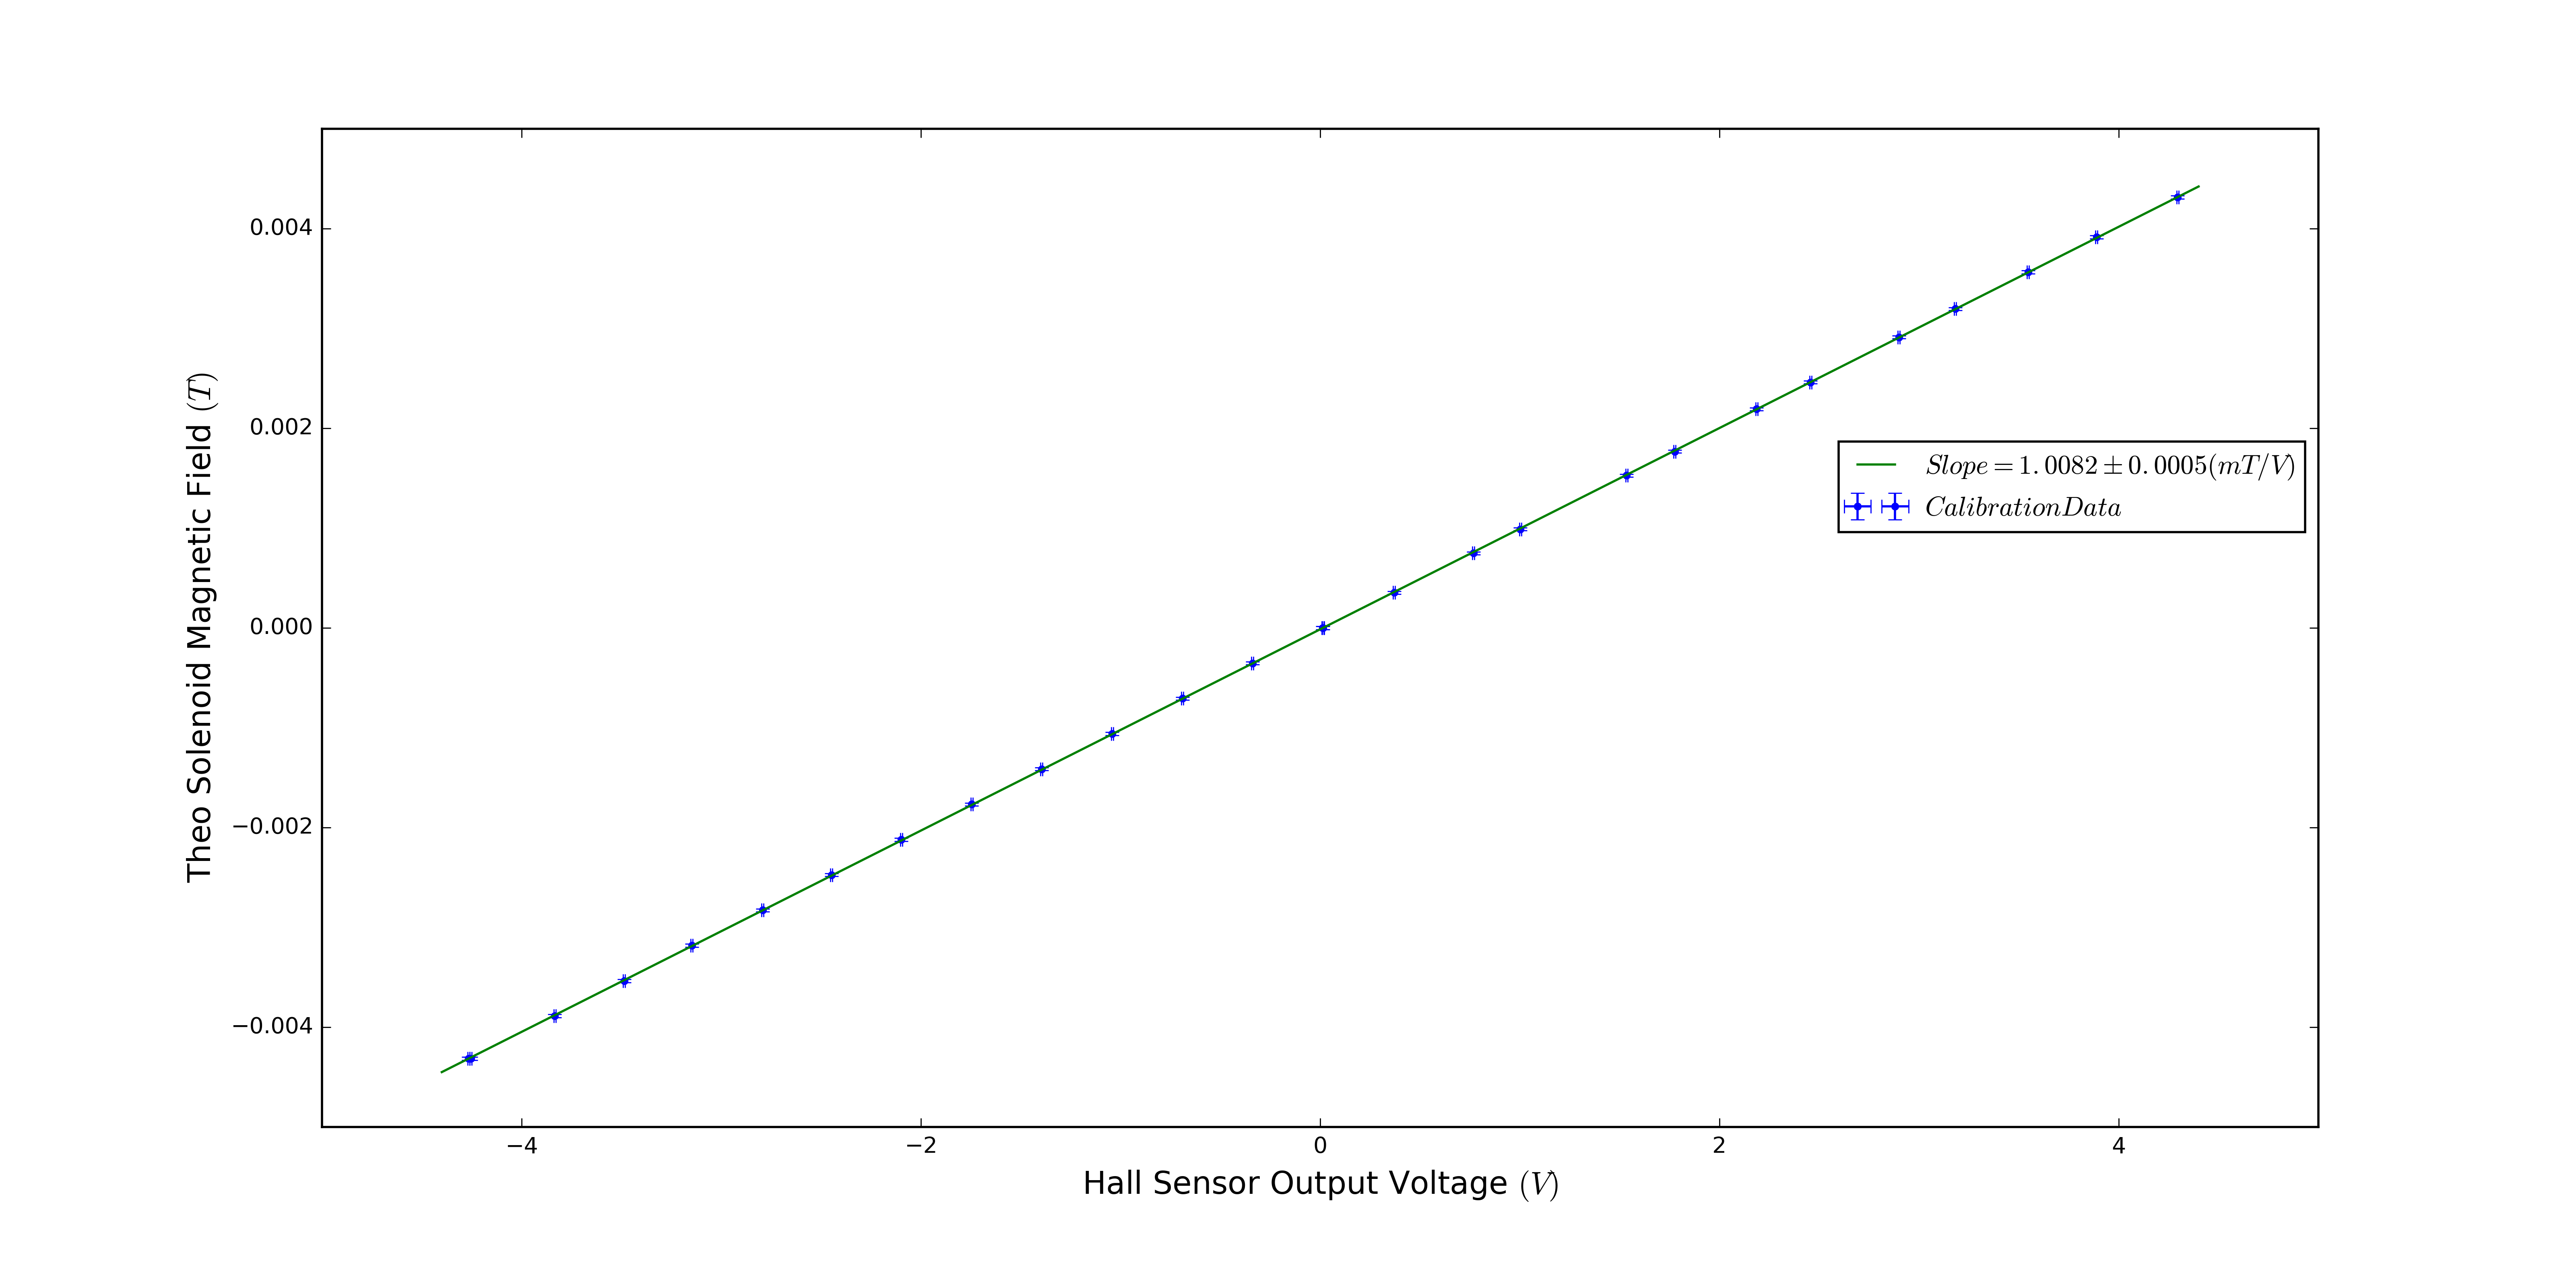
\includegraphics[height=0.70\textwidth]{../DataValidation/calibrationPlot}
\caption{The vertical axis corrisponds to the current we put through our solinoid. the error is in the curent uncertinty and uncertinty in measurements of the coil}
\label{apparatus}
\end{figure*}
\end{turnpage}

There are several ways to measure magnetic fields. since the invention of SQIDs (superconducting quantum interference devices) \ref art of electronics drinking glass page there are no methods more sensitive. however squids have a high entry cost and to maintain a liquid nitrogen setup to cool the apparatus is somewhat complicated. Hall-effect sensors can measure fields with 10\% accuracy and are extremely cheap. we wanted to explore the sensitivity, noise performance, linearity and gain of a TeachSpin analog output hall sensor. the sensor claimed a gain of 1 volt per Milli-Tesla. 
	To calibrate our probe we wound a solenoid \ref {table with solenoid dmms length, radius, turns, aspect ratio} Our calibration rides on the error in the current supplied to the solenoid, the dimensions of the solenoid as well as the field model of the solenoid: 
$$\vec B = \frac{\mu_0 N I}{L}$$ 
With the probe inserted [fraction of the length of the solenoid] into the solenoid, we took several measurements with a constant current supply [pm amps]. plotting the theoretical field as a function of the sensor's output allows us to obtain a gain of the sensor from a fit line slope, allows us to verify the linearity of the sensor in the range we intend to utilize in our next experiments. we found the senor to have a gain of: and we were able to measure the uncertainty in the calibration as: this combined with the uncertainty in our voltmeter will let us measure magnetic fields at: $\pm$ Milli-Tesla.


\section{Mapping the Helmholtz Field}
With our calibrated hall probe we measured the b field at different points allong the symetry  axis of the TeachSpin helmholtz coil pair. We modeled the theoretical field by deriving the onaxis field of one current loop and then taking a superposition of the field for each wire in the aparatus. the field for one loop of wire is:
$$\vec{B}=\frac{\mu_0}{2}\frac{I R_z^2}{\sqrt{R_y^2 + R_z^2}^3}$$
Where $R_z$ the radius of the loop and $R_y$ is the distance allong the axis of symetry away from the plane of the loop. 

With a Jupyter notebook we integrated each loop and plotted enough points to create our theoretical model. 

\begin{figure}[here]
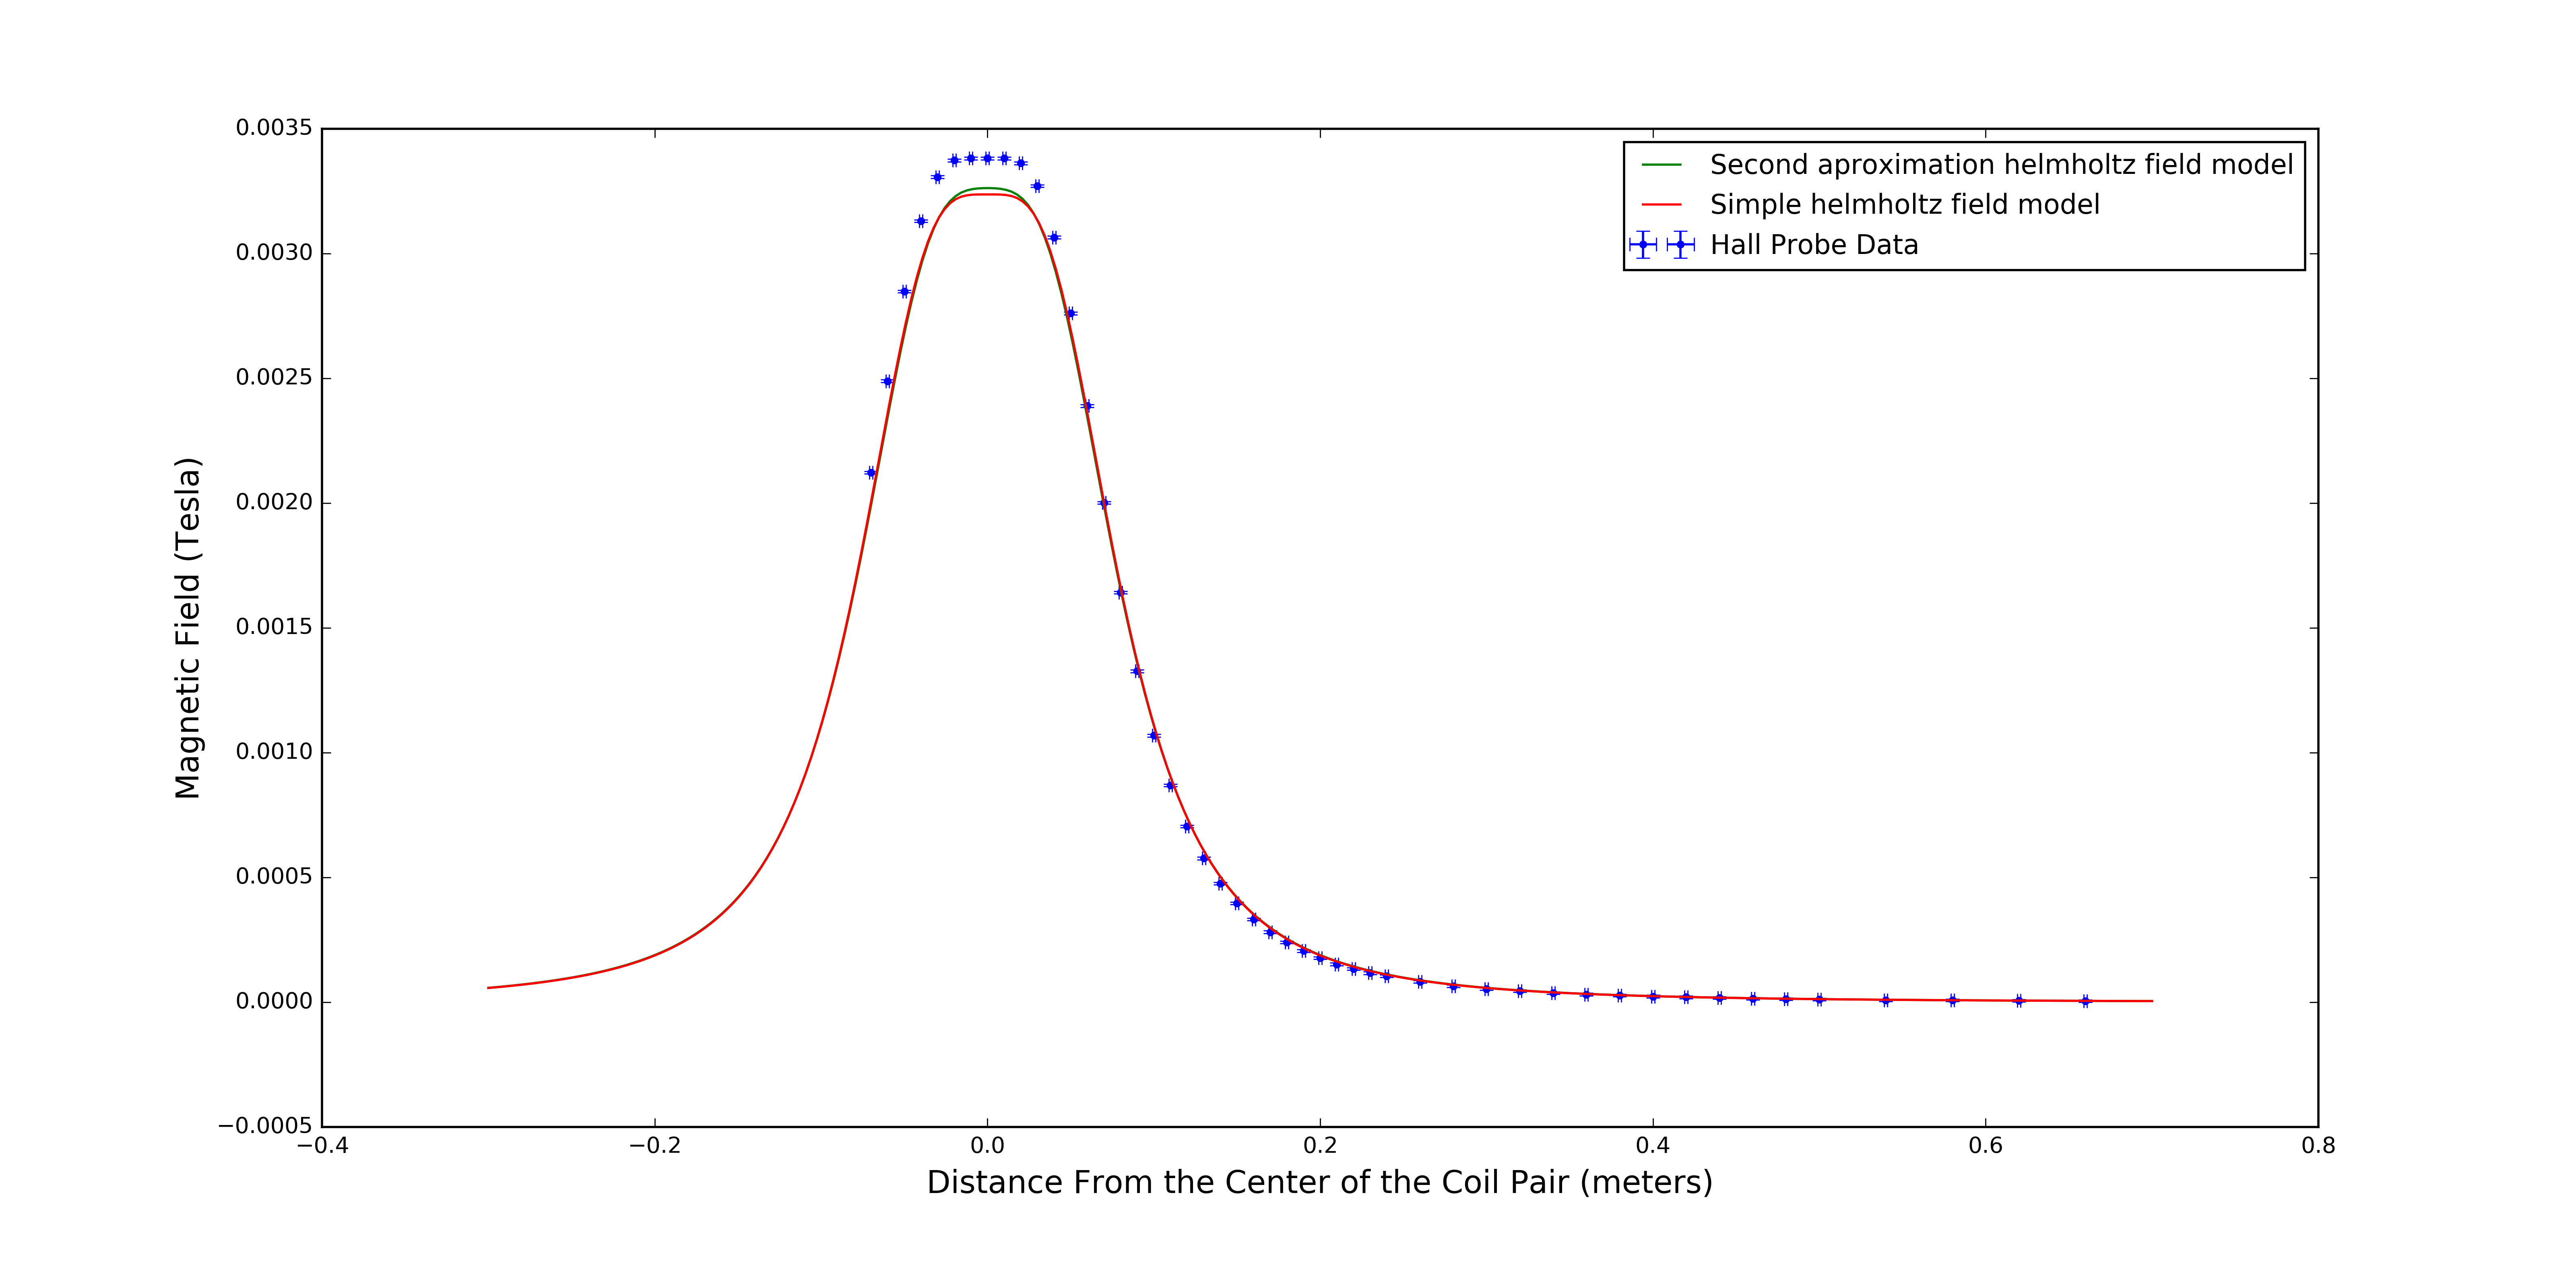
\includegraphics[width=1\textwidth]{../DataValidation/helmholtzPlot.png}
\caption{}
\label{apparatus}
\end{figure}

We also used the Helmholtz coils in quadrupole configureation. the field model is almost the same, we simmply reverse the field influence of the second coil. With the quadripole configureation, we can get a very uniform gradent field in the center of the coil pair, which alows us to verify that the force on a magnetic dipole is proportional to the gradent in the field. 



%Additionally, this gradent gets weaker on boundaries of the uniform poriton. If the frorce on a dipole is proportional to the gradent in the field, the center of the quadrupole field will be a stable equilibrium point. 

\begin{figure}[here]
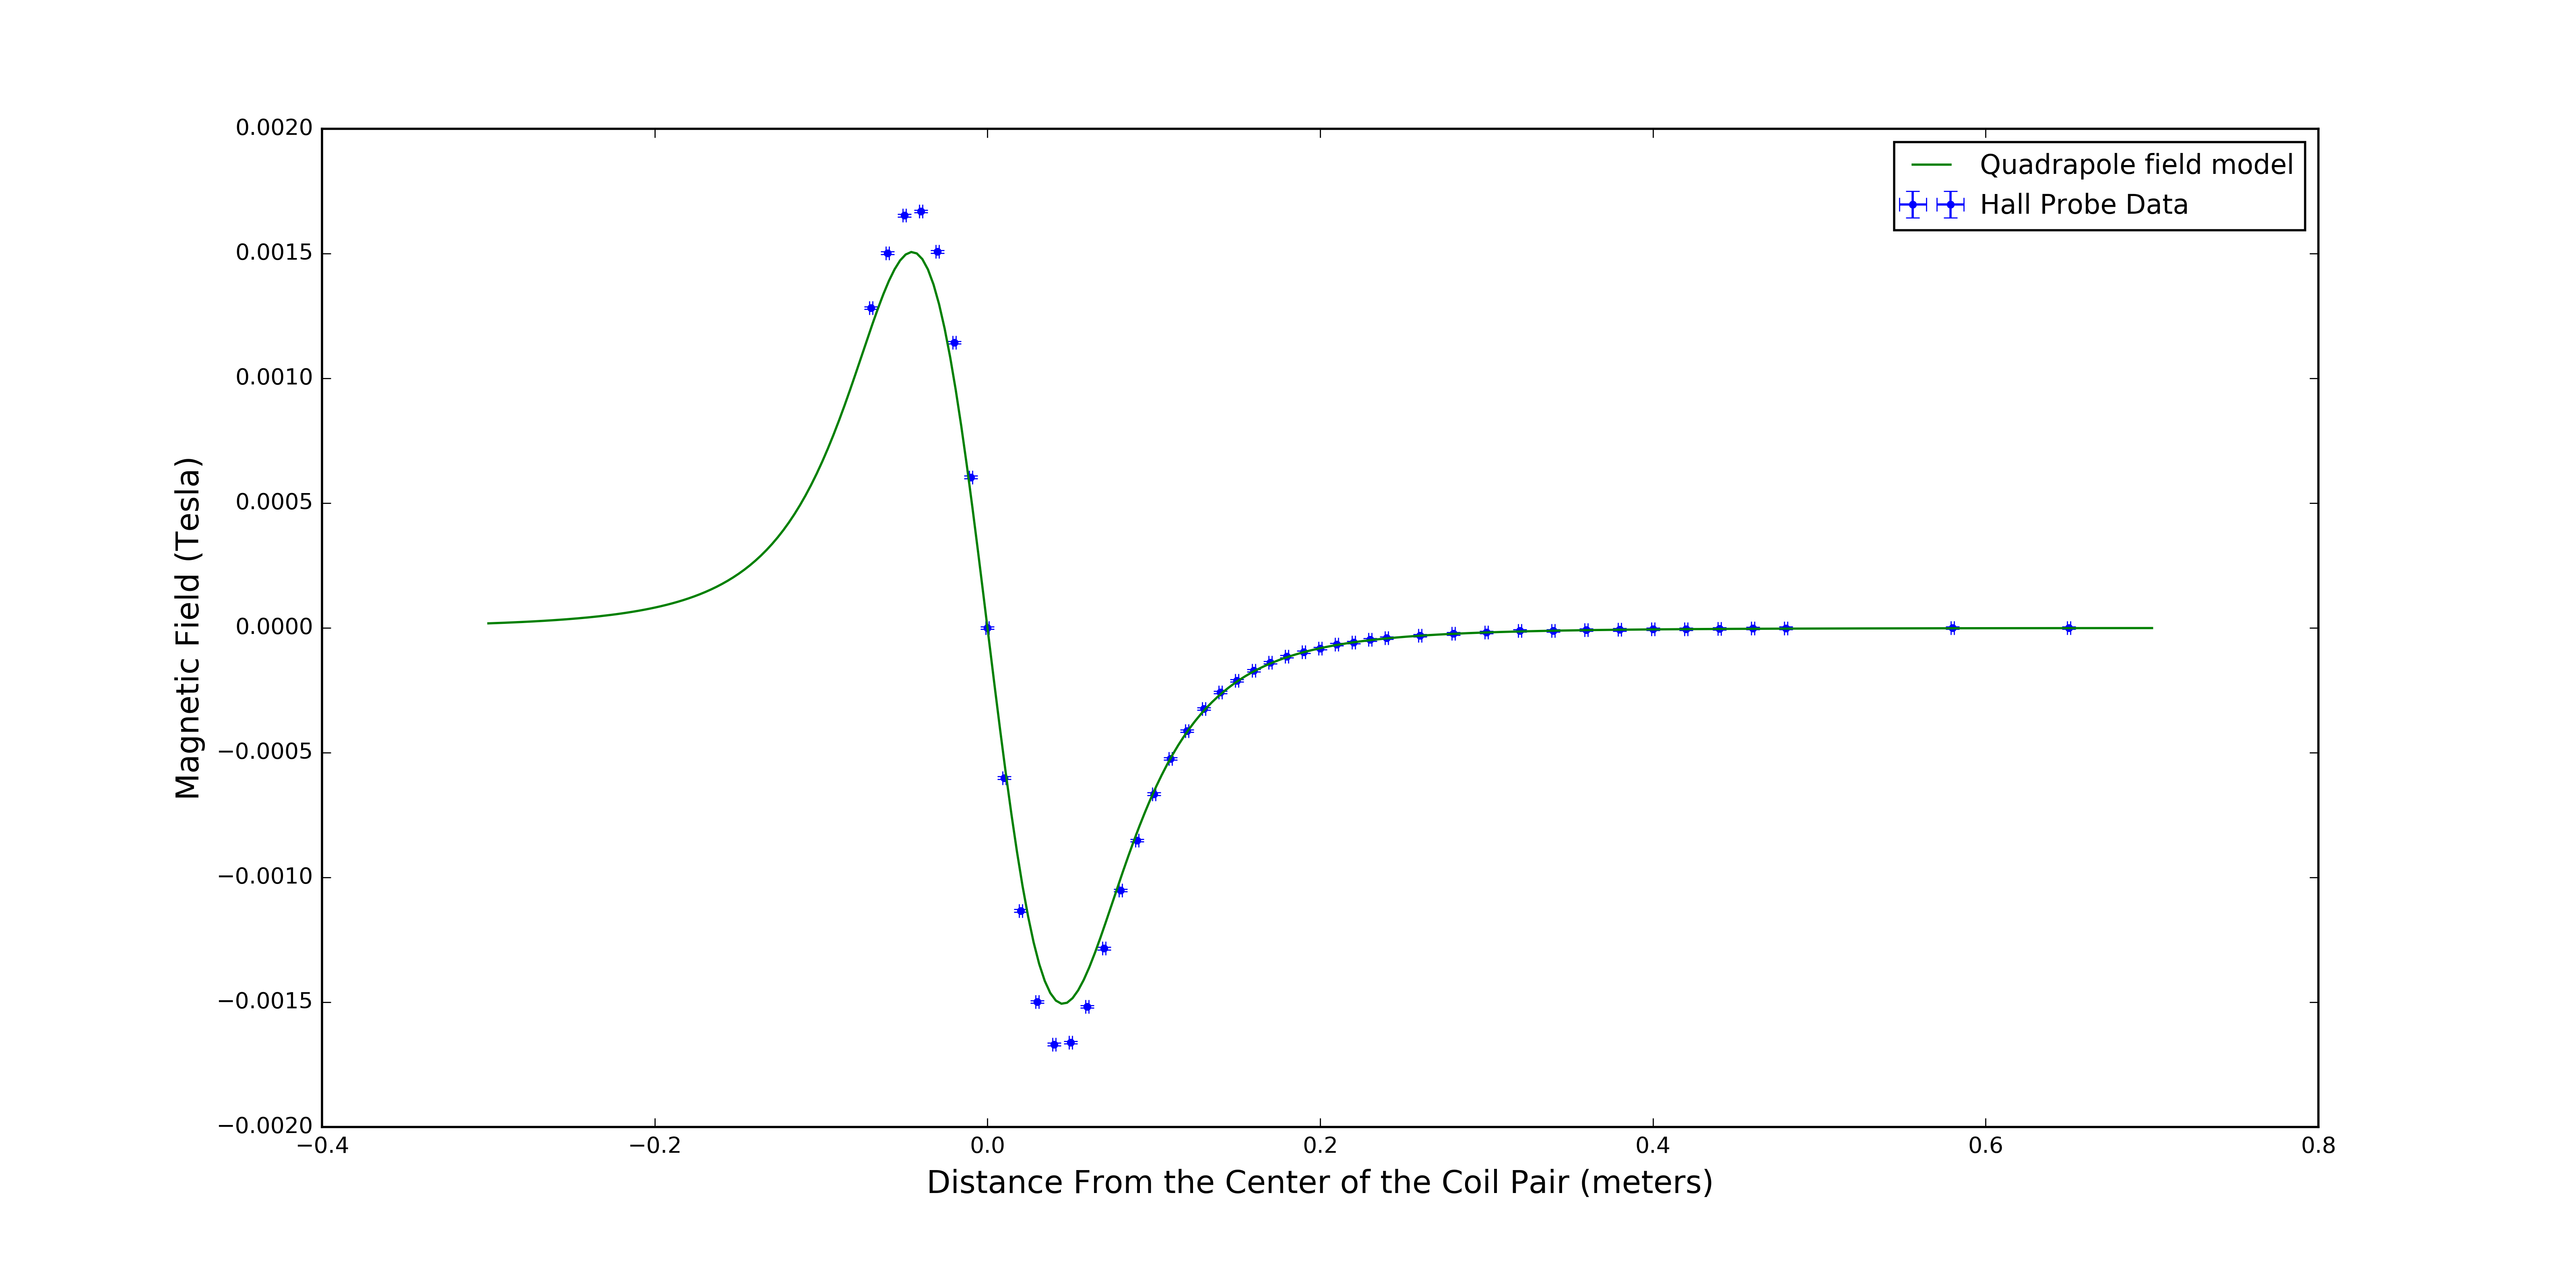
\includegraphics[width=1\textwidth]{../DataValidation/quadPlot.png}
\caption{}
\label{apparatus}
\end{figure}

\section{Force on a magnetic dipole}



















\begin{thebibliography}{9}

	
\bibitem{knight}
	Randall D. Knight
	\emph{Physics for Scientists and Engineers 3rd Edition}
	Pearson 2013
	
\bibitem{Higbie78}
	J. Higbie
	\emph{Off-axis Helmholtz field}
	American Journal of Physics 46, 1075 (1978)

	
	
\end{thebibliography}

\end{document}
